% The mean-field self-consistency loop, four steps with the mix-and-repeat back edge (Session 1).
% Own drawing (Fable). Compile with: pdflatex scf_loop.tex ; result moves to ../scf_loop.pdf
\documentclass[11pt,tikz,border=3pt]{standalone}
\usepackage{amsmath,amssymb}
\usepackage{xcolor}
\definecolor{coursedark}{HTML}{1B2A4A}
\definecolor{courseaccent}{HTML}{7A2E8C}

\begin{document}
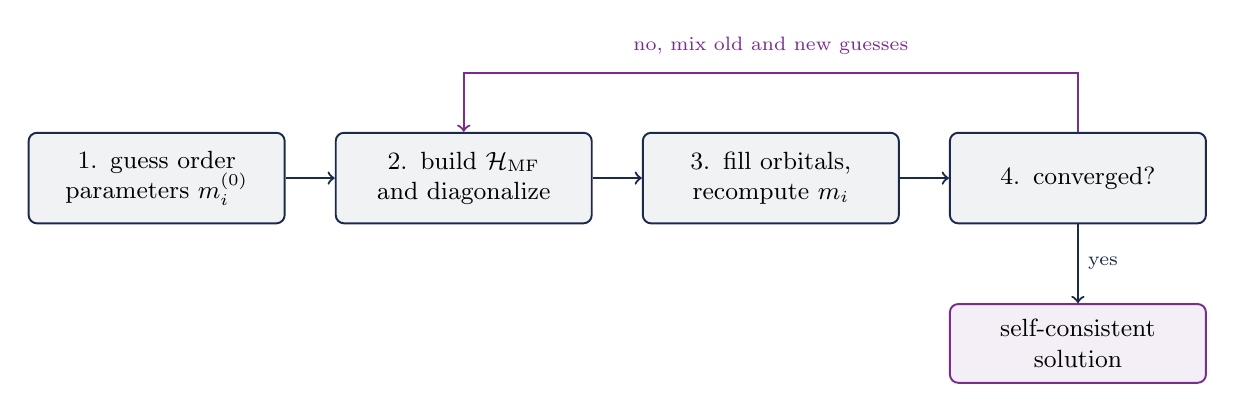
\begin{tikzpicture}[
    box/.style={draw=coursedark, fill=coursedark!6, rounded corners=3pt,
      line width=0.7pt, text width=2.9cm, align=center, font=\small,
      inner sep=5pt, minimum height=1.15cm},
    done/.style={draw=courseaccent, fill=courseaccent!8, rounded corners=3pt,
      line width=0.7pt, text width=2.9cm, align=center, font=\small,
      inner sep=5pt, minimum height=1.0cm},
    flow/.style={->, draw=coursedark, line width=0.8pt},
    idx/.style={font=\scriptsize, text=coursedark},
  ]

  \node[box] (n1) at (0,0)    {1. guess order parameters $m_i^{(0)}$};
  \node[box] (n2) at (3.9,0)  {2. build $\mathcal{H}_{\mathrm{MF}}$ and diagonalize};
  \node[box] (n3) at (7.8,0)  {3. fill orbitals,\\ recompute $m_i$};
  \node[box] (n4) at (11.7,0) {4. converged?};

  \draw[flow] (n1) -- (n2);
  \draw[flow] (n2) -- (n3);
  \draw[flow] (n3) -- (n4);

  \node[done] (n5) at (11.7,-2.1) {self-consistent solution};
  \draw[flow] (n4) -- (n5) node[idx, midway, anchor=west] {yes};

  \draw[->, courseaccent, line width=0.8pt]
    (n4.north) -- ++(0,0.75) -| (n2.north);
  \node[idx, text=courseaccent, anchor=south] at (7.8,1.45)
    {no, mix old and new guesses};
\end{tikzpicture}
\end{document}
